\documentclass[mres, copyrightpage, examinerscopy]{mqthesis}
%----------------------------------------------------------
% OPTIONS
% Options you can use in the documentclass above:
%
% phd/mres/hons = set the degree text [default=phd if absent]
% copyrightpage = print a copyright page on the back 
%                 of the title page [default=false]
% examinerscopy = print "Examiner's Copy" of title page and 
%                 change linespacing to 1.5 [default=false]
% greychapternumbers = print large chapter numbers in grey
%                 instead of MQ corporate "sand"
%---------------------------------------------------------- 

% this shows what labels you are using for cross references
% \usepackage{showkeys} 

%---------------------------------------------------------- 
% STRUCTURE
% this document is a skeleton which pulls in the meat of the thesis
% from other files. Comment out and add lines as appropriate.
%---------------------------------------------------------- 

% N.B. for final printing you may want to remove the 'examinerscopy' 
% option, which will remove 'Examiner's Copy' from title page
% and change the linespacing to single space for a professional look
% ... just saying. Check figure placement though!

\begin{document}

%---------------------------------------------------------- 
% FRONT
% Acknowledgements, titlepage, abstract, list of publications
%---------------------------------------------------------- 
\frontmatter

\title{Insert thesis title here}
\author{Insert your name here}
\department{Physics}  % put your department here

\titlepage

\chapter{Acknowledgements}

I would like to thank my wife Gazala who supported me and pushed me to do more astronomy and apply to the Master's program at Macquarie University. I would also like to thank my family in Sri Lanka who support everything I do and encouraged me to follow my interests no matter what. I would not be completing this work if not for my family.

A big thank you to my supervisor Dr Daniel Zucker who in addition to providing valuable feedback, guided and believed in me every step of the way. Your friendship and mentorship has made this journey so much more enjoyable. Thank you to Dr Ben Montet at UNSW who introduced me to the astronomy community in Australia and encouraged me to apply to Macquarie University. As an immigrant and someone who had no formal training in astronomy until this point, I owe a debt of gratitude.

Many thanks to Dr Sarah Martell at UNSW for the early feedback and guidance on P Cygni spectra. Thank you to Dr Gregor Traven at Lund University for his valuable feedback and sanity checks towards the end of the project. Thanks to Arv Hughes, Dr Sven Buder and Dr Klemen Čotar and the various members of the GALAH science team and HDR cohort at Macquarie University who provided feedback and support during various forums and meetings throughout the last year - your kindness, generosity and camaraderie is highly appreciated. Finally, many thanks to all my friends, particularly Nuzhi Meyen in Sri Lanka for his input on the mathematics of machine learning and my many friends in Sydney who have had to endure me talking about astronomy 24/7/365.
\chapter{List of Publications}

\begin{itemize}
\item[$\bullet$] insert author list \emph{insert paper title}.  (submitted to
	insert journal name)
\item[$\bullet$] insert author list \emph{insert paper title}.  
        insert journal name \textbf{insert volume number}, 
        insert article or page number (insert year)
\end{itemize}

\chapter{Abstract}

This is my abstract.  This is what I've spent the last $x$ years working on,
and I'm going to tell you about now.


\tableofcontents
% comment out these as required for your discipline
\listoffigures
\listoftables

%---------------------------------------------------------- 
% MAIN
% include chapters as neededlmodern
%---------------------------------------------------------- 
\mainmatter

% Introduction
\begin{savequote}[45mm]
When theory and experiment agree, 
that is the time to be especially suspicious. 
\qauthor{Niels Bohr}
\end{savequote}

\chapter{Introduction}


P-Cygni type stars exhibit P Cygni profiles, which are spectral components that show characteristic absorption, emission and wide absorption sub-components. Depending on the location of the foremost absorption component (either blue- or redshifted), P Cygni profiles can be subdivided into two classes: namely P Cygni, and the  redshifted counterpart inverse P Cygni (). Stars that exhibit these profiles in their spectra are considered to have two components and processes that contribute to these spectral lines (\cite{zhang2021catalog}). \cite{1953PDAO....9....1B}



% Other chapters in here
\chapter{Another Chapter}

It's likely that you'll need another chapter, so here's a filler just to see
where it will go \cite{sample}.


% Conclusion
\begin{savequote}[45mm]
If cats looked like frogs we'd realize what nasty, cruel little bastards they are. Style. That's what people remember.
\qauthor{Terry Pratchett}
\end{savequote}

\chapter{Conclusion}

Not a very interesting conclusion, however you'll need one for your thesis.




%---------------------------------------------------------- 
% APPENDICES
% include chapters as needed (will be numbered differently)
%---------------------------------------------------------- 
\appendix

\chapter{Appendix}

\section{Appendix C - Chapter 6}

\begin{table}[!htb]
\begin{center}
\begin{tabular}{|l|l|}
\hline
\textbf{count} & 7067.000000 \\ \hline
\textbf{mean} & 0.532952 \\ \hline
\textbf{std} & 0.444046 \\ \hline
\textbf{min} & 0.220042 \\ \hline
\textbf{25\%} & 0.280778 \\ \hline
\textbf{50\%} & 0.388232 \\ \hline
\textbf{75\%} & 0.562633 \\ \hline
\textbf{max} & 5.055410 \\ \hline
\end{tabular}
\caption{EW distribution summary statistics for emission-line stars identified in GALAH DR3}
\label{table:draglift1}
\end{center}
\end{table}

\begin{table}[!htb]
\begin{center}
\begin{tabular}{|l|l|}
\hline
\textbf{count} & 10364.000000 \\ \hline
\textbf{mean} & 0.539950 \\ \hline
\textbf{std} & 0.420590 \\ \hline
\textbf{min} & 0.250070 \\ \hline
\textbf{25\%} & 0.298572 \\ \hline
\textbf{50\%} & 0.392470 \\ \hline
\textbf{75\%} & 0.592625 \\ \hline
\textbf{max} & 5.369496 \\ \hline
\end{tabular}
\caption{EW distribution summary statistics for emission-line stars identified by Čotar et al. (various surveys).}
\label{table:draglift1}
\end{center}
\end{table}

\begin{figure}[!htb]
\centering
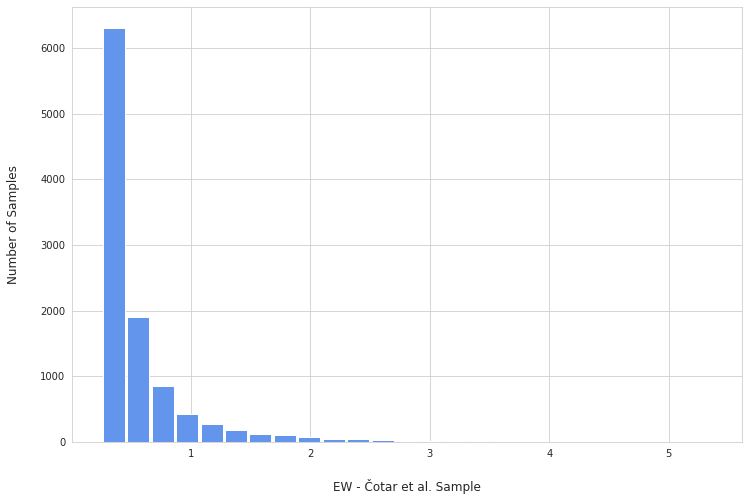
\includegraphics[scale=0.50]{figures/EW hist cotar.png}
\caption{The equivalent width (EW) distribution of the inverted difference spectra of the emission-line spectra provided by Čotar et al. Here EW > 0.25. Note that this sample contains additional spectra not in GALAH DR3.}
\end{figure}






%---------------------------------------------------------- 
% BACK
% list of symbols / references / index etc
%---------------------------------------------------------- 
\backmatter

% your thesis may not need this, so comment out or delete the following line
\chapter{List of Symbols}

% please change this list to suit your thesis

The following list is neither exhaustive nor exclusive, but may be helpful.
\begin{list}{}{%
\setlength{\labelwidth}{24mm}
\setlength{\leftmargin}{35mm}}
\item[$a$, $b$, $c$, $d$\dotfill] annihilation operators
\item[$a^\dagger$, $b^\dagger$, $c^\dagger$, $d^\dagger$\dotfill] creation
operators
\end{list}


% Bibliography, in BibTeX format (the references.bib file)
\bibliography{references}

\end{document}
